\documentclass{article}
\usepackage{listings}
\usepackage{mathrsfs}
\usepackage[utf8]{inputenc}
\usepackage{amssymb}
\usepackage{lipsum}
\usepackage{amsmath}
\usepackage{fancyhdr}
\usepackage{geometry}
\usepackage{scrextend}
\usepackage[english,german]{babel}
\usepackage{titling}
\setlength{\droptitle}{-3cm}
\usepackage{tikz}
\usepackage{algorithm,algpseudocode}
\usepackage[doublespacing]{setspace}
\usetikzlibrary{datavisualization}
\usetikzlibrary{datavisualization.formats.functions}
\usepackage{polynom}
\usepackage{amsmath}
\usepackage{gauss}
\usepackage{tkz-euclide}
\usetikzlibrary{datavisualization}
\usetikzlibrary{datavisualization.formats.functions}
\author{
Alexander Mattick Kennung: qi69dube\\
Kapitel 1
}
\usepackage{import}
\date{\today}
\geometry{a4paper, margin=2cm}
\usepackage{stackengine}
\parskip 1em
\newcommand\stackequal[2]{%
  \mathrel{\stackunder[2pt]{\stackon[4pt]{=}{$\scriptscriptstyle#1$}}{%
  $\scriptscriptstyle#2$}}
 }
\makeatletter
\renewcommand*\env@matrix[1][*\c@MaxMatrixCols c]{%
  \hskip -\arraycolsep
  \let\@ifnextchar\new@ifnextchar
  \array{#1}}
\makeatother
\lstset{
  language=haskell,
}
\lstnewenvironment{code}{\lstset{language=Haskell,basicstyle=\small}}{}
\usepackage{enumitem}
\setlist{nosep}
\usepackage{titlesec}

\titlespacing*{\subsection}{0pt}{2pt}{3pt}
\titlespacing*{\section}{0pt}{0pt}{5pt}
\titlespacing*{\subsubsection}{0pt}{1pt}{2pt}
\title{Vorlesung 4}


\begin{document}
	\maketitle
	große Varianz über fließkommaungenauigkeit führt bei stark schwankenden funktionen zu großen ungenauigkeiten! (spez. bei iterativen verfahren).\\
	\[\int_0^1 x^ne^{0.1x} dx\]
	Der fehler wird durch jeden iterationsschritt durchpropagiert und dadurch verstärkt!\\
	Idee:\\
	Rückwärtsiteration: $I_n = 10e^{0.1}-10n*I_{n-1}$\\
	$I_{n-1} = \frac{10e^{0.1}}{10n}$
	man beginnt bei schätzwert $\tilde I_{10}$\\
	und läuft davon rückwärts.\\
	je besser der schätzwert, desto schneller die Konvergenz, man kann z.B immer, wenn n ausgerechnet werden soll $I_{n+10} =0$ schätzen und dann 10 mal rückwärts approximieren. Wenn man bessere entwicklungszahl für $I_{n+k}$ hat braucht man vllt keine 10 schritte.\\
	Algorithmen, die fehler verstärken heißen \textbf{instabil.}
	Algorithmen, die dies nicht tun heißen \textbf{stabil}\\
	``Curse of dimensionality'', man versucht die eingangsdimensionalität zu minimieren.
	\section{Lin ALg}
	Lösen iterativ für große sparse matrices. evtl nie genauer Wert, keine feste iterationszahl\\
	Lösen direkt für kleine, exakte matrizen und lösungen. exakte Lösung(bis auf float-fehler), feste anzahl schritte e.g. $O(n^3)$\\
	direkt: Gauss-verfahren\\
	direkt: Faktorisieren $Ax=b\to A=A_1A_2$\\
	Dann leichtere lösen; $A_1y=d$ und $A_2 z=e$ also erst $A_1y=b$ lösen und dann in $A_2 x=y$
	LR-Zerlegung $A=LR$ wobei L eine (linke) untere Dreiecksmatrix und R eine (rechte) obere Dreiecksmatrix ist (LU-Decomposition)\\
	QR-Zerlegung $A=QR$, Q ist eine orthogonale matrix, R eine (rechte) obere Dreiecksmatrix.\\
	Eine nxn Matrix heißt orthogonal, falls eine dieser bedingungen gilt:\\
	$Q^TQ=Id$\\
	$QQ^T =Id$ (also $Q^{-1} =Q^T$\\
	Spalten oder Zeilen von Q bilden eine Orthonormalbasis\\
	Abbildung Q ist winkel und längentreu\\
	$Q$ erhält das skalarprodukt $Qx\circ Qy = x\circ y$\\
	Winkel $cos(x,y) = \frac{x\circ y}{||x|| ||y||}$\\
	Orthogonale Matritzen sind Drehungen oder Spiegelungen.\\
	$R=\begin{bmatrix} cos(\phi) &-sin(\phi)\\sin(\phi)&cos(\phi)\end{bmatrix}$\\
	$S = \begin{bmatrix} cos(2\phi) &sin(2\phi)\\sin(2\phi)&-cos(2\phi)\end{bmatrix}$
	Rückwärtsiteration von dreiecksmatrix $O(n^2)$\\
	Wenn man eine orthonormale Matrix Q hat auch $O(n^2)$ (das invertieren braucht halt $Q^{-1}=Q^T$ $n^2$ schritte zum umkopieren)\\
	Man kann die Matrix $Q$ in der Praxis auch nur die Rotationswinkel $\phi$ speichern.\\
	Die Inverse Abbildung kann die drehungen dann einfach in umgekehrter Reihenfolge durchführen.\\
	Wie kann man die Matrix A faktorisieren?\\
	$A=LR$ bzw $A=QR$ welche algorithmen/wie schnell?\\
	Der klassische Gauss mit Zeilenoperationen mit Ziel die  Dreiecksgestalt zu bekommen.\\
	Zeilenoperationen ergeben sich durch Multiplikation mit geeigneten Matritzen sog. Gauß-Scherungen.\\
	Einheitsmatrix mit einem $\alpha\neq 0$ irgendwo in der Matrix $N_{i,j}(\alpha)$:\\
	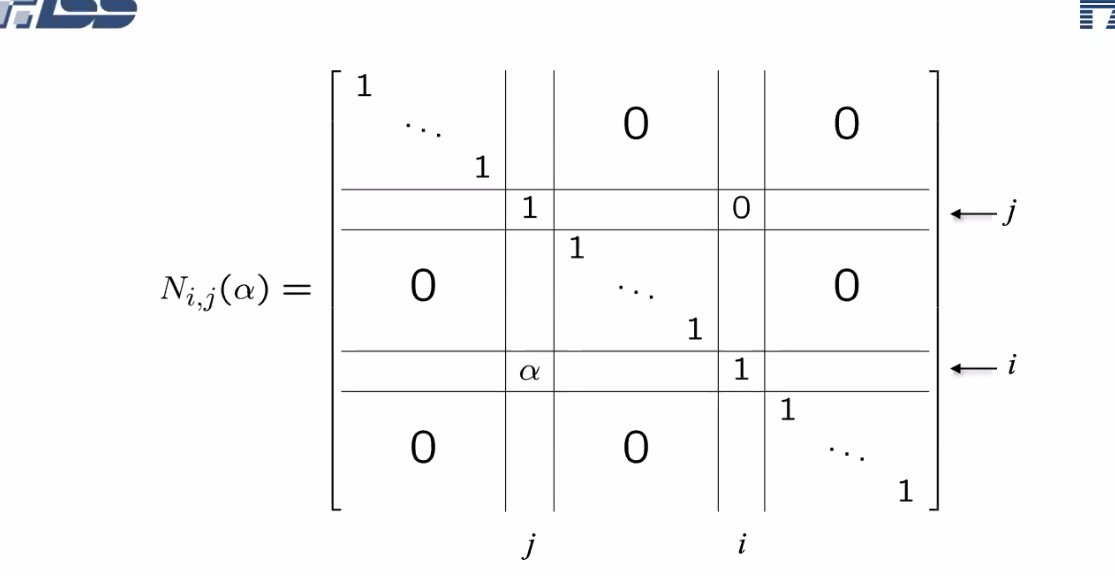
\includegraphics{guass-scherung.png}\\
	multipliziern mit einer solchen matrix fungiert als ``Zeilenadditionen''\\
	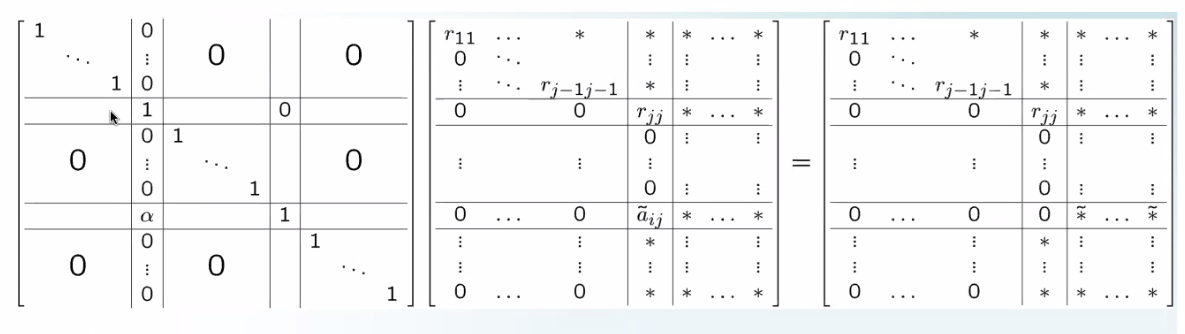
\includegraphics{multiplizierenMatrixenScherungen.png}\\
	$\alpha = \frac{-a_{i,j}}{a_{j,i}}$ wobei r das pivot element ist.\\
	
\end{document}